%
% Tesi D.S.I. - modello preso da
% Stanford University PhD thesis style -- modifications to the report style
%
%%%%%%%%%%%%%%%%%%%%%%%%%%%%%%%%%%%%%%%%%%%%%%%%%%%%%%%%%%%%%%%%%%%%%%%%%%%
%                                                                         %
%			TESI DOTTORATO                                                   %
%			______________                                                   %
%                                                                         %
%			AUTORE: Elena Pagani                                             %
%                                                                         %
%			Ultima revisione: 7.X.1998                                       %
%           correzioni atrent                                             %
%%%%%%%%%%%%%%%%%%%%%%%%%%%%%%%%%%%%%%%%%%%%%%%%%%%%%%%%%%%%%%%%%%%%%%%%%%%
%
%
\documentclass[a4paper,12pt]{report}
%\renewcommand{\baselinestretch}{1.6}      % interline spacing
%
% \includeonly{}
%
%			PREAMBOLO
%
\usepackage[a4paper]{geometry}
\usepackage{microtype}
\usepackage{amssymb,amsmath,amsthm}
\usepackage{graphicx}
\usepackage{url}
\usepackage{epsfig}
\usepackage[italian]{babel}
\usepackage{setspace}
\usepackage{tesi}
\usepackage{nameref}
\usepackage[italian]{varioref}
\usepackage{footnotebackref}
\usepackage{hyperref}
\usepackage{caption}
\usepackage{subcaption}
\usepackage{pgfplots}
\usepackage{tikz}
\usepackage{minted}
\usepgfplotslibrary{fillbetween}
\pgfplotsset{width=10cm,compat=1.9}
\emergencystretch=100em


% \captionsetup{width=1\textwidth,font={small, sl},labelfont={bf}}


% per le accentate
\usepackage[utf8]{inputenc}
% \graphicspath{.\Images}
%
\newtheorem{myteor}{Teorema}[section]
%
\newenvironment{teor}{\begin{myteor}\sl}{\end{myteor}}
%
%
%			TITOLO
%
% \includegraphics{Logo}
\begin{document}
\title{Implementazione e confronto di algoritmi di ottimizzazione per l'apprendimento di insiemi fuzzy}
\author{Giacomo Intagliata}
\dept{Corso di Laurea Triennale in Informatica} 
\anno{2020-2021}
\matricola{873511}
\relatore{Prof. Dario MALCHIODI}
\correlatore{Prof. Alberto CESELLI}
%
%        \submitdate{month year in which submitted to GPO}
%		- date LaTeX'd if omitted
%	\copyrightyear{year degree conferred (next year if submitted in Dec.)}
%		- year LaTeX'd (or next year, in December) if omitted
%	\copyrighttrue or \copyrightfalse
%		- produce or don't produce a copyright page (false by default)
%	\figurespagetrue or \figurespagefalse
%		- produce or don't produce a List of Figures page
%		  (false by default)
%	\tablespagetrue or \tablespagefalse
%		- produce or don't produce a List of Tables page
%		  (false by default)
% 
%			DEDICA
%
\beforepreface
% \prefacesection{}
%          {\hfill \Large {\sl dedicato a \dots}}

% %
%
%			RINGRAZIAMENTI
%
% \prefacesection{Ringraziamenti}
% asdjhgftry.
\afterpreface

%
\chapter*{Introduzione}
\addcontentsline{toc}{chapter}{Introduzione}
\label{Introduzione}
%
Come è strutturata la tesi.
% 

%			CAPITOLO 1: descrizione problema da affrontare

\chapter{Insiemi fuzzy e Machine Learning}
\label{Capitolo 1}
\section{Logica fuzzy}
La logica fuzzy \cite{logica_fuzzy} è un'estensione della logica booleana.
Nella logica booleana i predicati logici che vengono valutati possono assumere solo i valori \textit{vero} o \textit{falso}, generalmente codificati in ambito informatico con 1 e 0.


La logica fuzzy, a differenza della logica booleana, è in grado di trattare contesti ambigui e non esattamente definiti.
Nella logica fuzzy i predicati logici possono assumere valori compresi nell'intervallo $[0,1]$, dove gli estremi corrispondono rispettivamente a \textit{falso} e \textit{vero}.
Il valore assunto è chiamato \textit{valore di appartenenza} o \textit{grado di verità}, e indica quanto è vera una proprietà, permettendo a un predicato di essere parzialmente vero o parzialmente falso, e non necessariamente completamente vero o completamente falso.

\bigskip

Per capire meglio questo concetto possiamo fare qualche esempio che rispecchia la vita reale, dove molte cose non vengono valutate in maniera netta e non sempre sono tutto o niente; si potrebbe per esempio dire che:


\begin{itemize}
    \item l'acqua che esce dal rubinetto è  \textit{fredda} con un grado di verità 0.4;
    \item un diciottenne è \textit{giovane} con un grado di verità 0.8;
    \item una persona di 180 cm è \textit{alta} con un grado di verità 0.7.
\end{itemize}

\noindent Nell'esempio in Figura \ref{fig:Differenze_Logiche} vediamo meglio come cambia la valutazione del predicato `\textit{L'acqua che esce dal rubinetto è fredda}' a seconda della logica considerata.

\begin{figure}
    \begin{subfigure}[t]{.46\textwidth}
        \centering
        \resizebox{6cm}{5cm}{
        \begin{tikzpicture}
            \begin{axis}[
                axis lines = left,
                xlabel = {Temperatura},
                ylabel = {Grado di verità},
                xmin=0, xmax=60,
                ymin=0, ymax=1.2,
            ]    
            \end{axis}    
            \draw[ultra thick,color=blue](0,5.87) -- node[below,yshift = -1cm, xshift = 2mm] {Fredda} ++ (3.5,0) -- (3.5,0) -- (8,0);    
            % \draw[ultra thick,color=red](0,0) -- (3.55,0) -- (3.55,5.87) -- node[below, yshift=-1cm] {Caldo} ++ (4.5,0);
        \end{tikzpicture}
        }
        \caption{Logica Booleana}
        \label{subfig:Logica_booleana}
    \end{subfigure}
    \quad
    \begin{subfigure}[t]{.5\textwidth}
        \centering
        \resizebox{6cm}{5cm}{
        \begin{tikzpicture}
            \begin{axis}[
                axis lines = left,
                xlabel = {Temperatura},
                ylabel = {Grado di verità},
                xmin=0, xmax=60,
                ymin=0, ymax=1.2,
            ]    
            \end{axis}    
            \draw[ultra thick,color=blue](0,5.87) -- node[below,yshift = -1cm, xshift = 2mm] {Fredda} ++ (2,0) -- (5,0) -- (8,0);    
            % \draw[ultra thick,color=red](0,0) -- (2,0) -- (5,5.87) -- node[below, yshift=-1cm] {Caldo} ++ (3,0);
        \end{tikzpicture}
        }
        \caption{Logica Fuzzy}
        \label{subfig:Logica_fuzzy_grafico}
    \end{subfigure}
    \caption{Valutazione del predicato `\textit{L'acqua che esce dal rubinetto è fredda}' a seconda della logica considerata. Nell'asse delle ascisse è rappresentata la temperatura in gradi C°, mentre nell'asse delle ordinate il grado di verità del predicato a seconda della temperatura considerata. Nel caso della logica booleana (\subref{subfig:Logica_booleana}) il grado di verità è 1 o 0 a seconda di dove fissiamo la soglia. Nel caso della logica fuzzy (\subref{subfig:Logica_fuzzy_grafico}) può essere utilizzata una generica funzione per determinare come il grado di verità decresca da 1 a 0.}
    \label{fig:Differenze_Logiche}
\end{figure}

\newpage

\section{Insiemi Fuzzy}
Quando il predicato `\textit{l'elemento $x$ appartiene all'insieme $A$}' non è  più valutato in termini di logica classica ma di logica fuzzy si dice che $A$ è un \textit{insieme fuzzy} \cite{logica_fuzzy}. 
Formalmente il grado di verità è determinato da un'opportuna \textit{funzione di appartenenza} `$\mu_A$'. Quindi volendo valutare un generico elemento $x$ di un universo del contesto $U$ avremo:
\begin{equation*}
    \mu_A(x) = \mu
\end{equation*}
%%SISTEMARE
%Nota che quando parli della funzione di appartenenza non va bene dire che x è un  predicato, perché si tratta di un generico elemento di un universo del discorso U
\noindent 
%La $x$ rappresenta i predicati da valutare ed appartenenti a un insieme di predicati $U$. 
dove la $\mu$ rappresenta il valore di appartenenza dell'elemento all'insieme fuzzy $A$ considerato ed è un valore reale compreso tra 0 e 1. 
Per $\mu_A(x)$ pari a 1 l’elemento è certamente incluso nell’ insieme, per $\mu_A(x)$ pari a 0
l’elemento non è per niente incluso nell’ insieme (questi due valori corrispondono alla teoria classica degli insiemi), mentre per tutti i valori compresi tra 0 e 1 l’appartenenza può essere più o meno forte.

\bigskip

Consideriamo per esempio l'universo $U$ di tutte le persone e un ipotetico insieme fuzzy $A$ di tutte le persone `giovani'. Per ognuno di questi elementi in $U$:
\begin{itemize}
    \item ottantenne;
    \item ventenne;
    \item neonato;
\end{itemize}
possiamo definire un grado di appartenenza all'insieme $A$. Per esempio:
\begin{itemize}
    \item l'ottantenne appartiene ad $A$ con un valore pari a 0.1;
    \item il ventenne appartiene ad $A$ con un valore pari a 0.8;
    \item il neonato appartiene ad $A$ con un valore pari a 1;
\end{itemize}
Possiamo formalizzare questo ragionamento.
Dato un universo $U$ si definisce un insieme fuzzy $A$ tramite la funzione di appartenenza $\mu_A$, la quale determina il grado di appartenenza ad $A$ per ogni elemento dell'insieme $U$:
\begin{equation*}
    \mu_A : U \to [0,1].
\end{equation*}

\subsection*{Operazioni tra insiemi fuzzy}
La teoria degli insiemi fuzzy è un'estensione della teoria classica degli insiemi, ovvero è una teoria che è inclusa in quella classica, ma allo stesso tempo la allarga.
\`E possibile estendere agli insiemi fuzzy gli operatori insiemistici classici: unione, intersezione e complemento. Esistono vari modi di definire questi operatori per gli insiemi fuzzy. 
%Uno di questi è definirli attraverso le funzioni di appartenenza dell'insieme fuzzy che si ottiene come risultato applicando le operazioni stesse.
Di seguito degli esempi, per ogni operatore, che mostrano come ottenere la funzione di appartenenza dell'insieme risultante a partire da quella degli operandi.

\bigskip
Definiamo due insiemi fuzzy, $A$ e $B$ (ad esempio come in Figura \ref{fig:Insiemi Fuzzy}) di un universo $U$. I paragrafi successivi contengono delle possibili definizioni delle operazioni di \textit{unione}, \textit{intersezione} e \textit{complemento}, calcolate sugli insiemi fuzzy appena definiti.

\begin{figure}[h]
    \begin{subfigure}[t]{0.47\textwidth}
        \centering
        \resizebox{6cm}{5cm}{
        \begin{tikzpicture}
            \begin{axis}[
                axis lines = left,
                ylabel = {Grado di appartenenza},
                xlabel = {$U$},
                ymin=0, ymax=1.2,
                xmin=0, xmax=21,
                xticklabels={,,},                
            ]

            \addplot [color = blue, name path=A, ultra thick] coordinates {
            (0,1)
            (7,1)
            (14,0)
            (21,0)}; 

            \end{axis}

        \end{tikzpicture}
        }
        \caption{Insieme $A$}
    \end{subfigure}
    \begin{subfigure}[t]{0.47\textwidth}
        \centering
        \resizebox{6cm}{5cm}{
        \begin{tikzpicture}
            \begin{axis}[
                axis lines = left,
                ylabel = {Grado di appartenenza},
                xlabel = {$U$},
                ymin=0, ymax=1.2,
                xmin=0, xmax=21,
                xticklabels={,,},                
            ]
            
            \addplot [color = red, name path = B, ultra thick] coordinates {
            (0,0)
            (7,0)
            (14,1)
            (17,0.5)
            (21,0.5)};           

            \end{axis}           

        \end{tikzpicture}
        }
        \caption{Insieme $B$}
    \end{subfigure}
    \caption{Grafico delle funzioni di appartenenza degli insiemi fuzzy utlizzati per esemplificare le principali operazioni tra insiemi fuzzy.}
    \label{fig:Insiemi Fuzzy}
\end{figure}

\subsubsection{Unione}
L'unione $A \cup B$ di due insiemi fuzzy $A$ e $B$ risulta essere anch'essa un insieme fuzzy in $U$, con una funzione di appartenenza, mostrata in Figura \ref{fig:Unione_Insiemi_Fuzzy}, pari a:
\begin{equation*}
    \mu_{A\cup B} (u) = \max\{\mu_A(u),\mu_B(u)\} \hspace{1cm}  \forall u\in U.
\end{equation*}

\begin{figure}[h]
    \centering
    \resizebox{6.16cm}{4.4cm}{
    \begin{tikzpicture}
        \begin{axis}[
            axis lines = left,
            ylabel = {Grado di appartenenza},
            xlabel = {$U$},
            ymin=0, ymax=1.2,
            xmin=0, xmax=21,
            xticklabels={,,},                
        ]
        \addplot [color = blue] coordinates {
        (0,1)
        (7,1)
        (14,0)
        (21,0)}; 
        
        \addplot [color = red] coordinates {
        (0,0)
        (7,0)
        (14,1)
        (17,0.5)
        (21,0.5)}; 

        \addplot [color = violet, ultra thick] coordinates {
            (0,1)
            (7,1)
            (10.5,0.5)
            (14,1)
            (17,0.5)
            (21,0.5)
        };
        \end{axis}

    \end{tikzpicture}
    }
    \caption{Unione tra insiemi fuzzy. In viola viene rappresentata la funzione di apparteneza dell'unione degli insiemi $A$ e $B$ mostrati in Figura \ref{fig:Insiemi Fuzzy}.}
    \label{fig:Unione_Insiemi_Fuzzy}   

\end{figure}

\subsubsection{Intersezione}
L'intersezione $A \cap B$ di due insiemi fuzzy $A$ e $B$ risulta essere anch'essa un insieme fuzzy di $U$, con una funzione di appartenenza, mostrata in Figura \ref{fig:Intersezione_insiemi_fuzzy}, pari a:
\begin{equation*}
    \mu_{A \cap B} (u) = \min\{\mu_A(u),\mu_B(u)\} \hspace{1cm}  \forall u\in U.
\end{equation*}

\begin{figure}[ht]
    \centering
    \resizebox{6.16cm}{4.4cm}{
    \begin{tikzpicture}
        \begin{axis}[
            axis lines = left,
            ylabel = {Grado di appartenenza},
            xlabel = {$U$},
            ymin=0, ymax=1.2,
            xmin=0, xmax=21,
            xticklabels={,,},                
        ]
        \addplot [color = blue] coordinates {
        (0,1)
        (7,1)
        (14,0)
        (21,0)}; 
        
        \addplot [color = red] coordinates {
        (0,0)
        (7,0)
        (14,1)
        (17,0.5)
        (21,0.5)}; 

        \addplot [color = violet, ultra thick] coordinates {
            (0,0)
            (7,0)
            (10.5,0.5)
            (14,0)
            (21,0)
        };
        \end{axis}

    \end{tikzpicture}
    }
    \caption{Intersezione tra insiemi fuzzy. In viola viene rappresentata la funzione di appartenenza dell'intersezione degli insiemi $A$ e $B$ mostrati in Figura \ref{fig:Insiemi Fuzzy}.}
    \label{fig:Intersezione_insiemi_fuzzy}   

\end{figure}

\subsubsection{Complemento}
Il complemento di un insieme fuzzy $A$ è a sua volta un insieme fuzzy indicato con $\neg A$ e con funzione di appartenenza, mostrata in Figura \ref{fig:Complemento_insieme_fuzzy}, pari a:
\begin{equation*}
    \mu_{\neg A}(u) = 1 - \mu_A(u) \hspace{1cm}  \forall u\in U.
\end{equation*}

\begin{figure}[ht]
    \centering
    \resizebox{6.16cm}{4.4cm}{
    \begin{tikzpicture}
        \begin{axis}[
            axis lines = left,
            ylabel = {Grado di appartenenza},
            xlabel = {$U$},
            ymin=0, ymax=1.2,
            xmin=0, xmax=21,
            xticklabels={,,},                
        ]
        \addplot [color = blue] coordinates {
        (0,1)
        (7,1)
        (14,0)
        (21,0)}; 

        \addplot [color = violet, ultra thick] coordinates {
            (0,0)
            (7,0)
            (14,1)
            (17,1)
            (21,1)};

        \end{axis}

    \end{tikzpicture}
    }
    \caption{Complemento di un insieme fuzzy. In viola viene rappresentato la funzione di appartenenza del complemento dell'insieme $A$ mostrato in Figura \ref{fig:Insiemi Fuzzy}.} 
    \label{fig:Complemento_insieme_fuzzy}  

\end{figure}


\section{Machine Learning}
Il Machine Learning \cite{machine_learning_oreilly} è una branca dell'informatica nella quale in una macchina si predispone l'abilità di apprendere qualcosa dai dati in maniera induttiva.
Metaforicamente, il Machine Learning permette ai computer di compiere attività imparando dall'esperienza (che in questo caso è costituita dai dati a disposizione). \newline
Gli algoritmi di Machine Learning migliorano le loro prestazioni in modo adattivo mano a mano che gli esempi da cui apprendere aumentano.

\bigskip
Gli algoritmi di Machine Learning differiscono tra loro a seconda dell'approccio utilizzato per apprendere a partire dai dati.
% \footnote{Esistono anche altri criteri che permettono di caratterizzare i diversi tipi di Machine Learning, ad esempio basati sui dati che utilizzano, che producono, o sul tipo di problema.\label{nota:tipi ml}}.
%riferimento biografico nota
Possiamo avere degli approcci di diverso tipo:
\begin{itemize}
    \item supervisionato;
    \item non supervisionato;
    \item semi-supervisionato;
    \item apprendimento con rinforzo.
\end{itemize}

\noindent In seguito vediamo nel dettaglio come differiscono questi approcci.

\subsection*{Approccio Supervisionato}
L'\textit{Approccio Supervisionato} \cite{machine_learning_oreilly}\cite{unsupervised_learning} è una tecnica di apprendimento automatico che punta a istruire una macchina lavorando su un insieme di dati associati a etichette definite dall'utente.
Come abbiamo già detto, gli algoritmi di Machine Learning apprendono da esempi, questi nell'approccio supervisionato sono costituiti da coppie composte da istanze del problema e dalla loro soluzione, e quest'ultima è spesso codificata con delle etichette definite dall'utente. 
%Per esempio nella classificazione avremo un'etichetta per ogni classe da considerare.
%Istriuire una macchina (?). Prima abbiamo detto che ci sono questi esempi utilizzati, nell'approccio supervisionato questi esempi sono delle coppie, l'istanza di un problema e la sua soluzione, codificata spesso con delle etichette definite dall'utente

% L' approccio supervisionato è una tecnica di apprendimento automatico che mira ad istruire un sistema informatico in modo da consentirgli di elaborare automaticamente previsioni sui valori di uscita di un sistema rispetto ad un input sulla base di una serie di esempi ideali, costituiti da coppie di input e di output, che gli vengono inizialmente forniti.
% Questa tecnica lavora su un insieme di dati associati ad etichette definite dall'utente. 
Sapendo che ogni dato è associato a un'etichetta si vuole arrivare a cogliere la relazione che vi è tra dati ed etichette, così da poter predire le etichette anche a partire dai dati non visti durante la fase di apprendimento. 
In questo approccio è possibile lavorare con etichette di tipi diversi, sia discreti che continui.
In output da un algoritmo di apprendimento automatico abbiamo quello che viene chiamato modello. 
% Questa tecnica può fornire due diversi tipi di risultati: discreti o continui. 


%%%%% 

Per fare un esempio, consideriamo delle diagnosi mediche fatte su una serie  di pazienti. 
Analizzando le diagnosi un medico è in grado di definire se il paziente è in salute o meno. Da qui possiamo estrapolare quindi due etichette differenti per il nostro caso: `in salute' e `malato'. 
In questi contesti si parla di classificazione, perché dato un oggetto voglio associarlo a una fra un numero ristretto di etichette, dove ogni etichetta rappresenta una classe, mentre il modello prende il nome di classificatore. Nel caso dell'esempio le due classi sono quelle del paziente `in salute' e del paziente `malato'. 

% Si chiamano classificatori quei sistemi che sono in output ad un algoritmo di apprendimento supervisionato basato su etichette di questo tipo.
Fornendo come input a un classificatore questo insieme di dati con le rispettive etichette appena definite, il calcolatore, tramite un algoritmo supervisionato, sarà in grado di fornire delle predizioni sulla possibile etichetta da attribuire a ogni nuova diagnosi.
Però è necessario che vi siano molti dati da analizzare, perché quando questo non succede la capacità di predizione del sistema che si ottiene è spesso di bassa qualità.

Nell'esempio precedente abbiamo utilizzato solamente le classi `in salute' e `malato', ma se volessimo quantificare l'aspettativa di vita non sarebbe più possibile ricorrere ai classificatori. Nasce quindi la necessità di passare da un'etichetta discreta a una continua, pertanto si utilizzano i \textit{regressori} che costituiscono un modello per predire valori continui.
Ad esempio, potremmo voler quantificare, data una specifica diagnosi, il tempo di guarigione per un paziente malato che per definizione si definisce su una scala numerica (ad esempio il numero di giorni).

Per riuscire a eseguire una predizione su dati nuovi, mai visti prima, con precisione accettabile, dobbiamo assicurarci che non si verificano due condizioni note come il sovra-adattamento (\textit{overfitting}) e il sotto-adattamento (\textit{underfitting}).

%parlare di modello all'inizo

L’\textit{overfitting} si verifica quando il modello tende ad adattarsi in maniera eccessiva ai dati che gli sono stati forniti per l'apprendimento (insieme denominato \textit{training set}), non permettendo la generalizzazione a nuovi insiemi di dati. L’\textit{underfitting}, invece, si verifica nel caso contrario, ovvero quando il modello si basa su schemi troppo semplici e poco robusti, il che comporta una scarsa qualità per la predizione degli elementi.

Quello che vogliamo è trovare un modello che si posizioni tra l'\textit{overfitting} e l' \textit{underfitting}.
Normalmente un modello è caratterizzato da un certo numero di parametri che devono essere opportunamente dimensionati durante l'apprendimento.
Il numero di questi parametri è un aspetto chiave da considerare.
Utilizzando un numero basso di parametri si rischia di ottenere modelli poco significativi, mentre utilizzandone troppi rischiamo di non concentrarci sui parametri davvero significativi nonché ricadere nel problema dell'overfitting.

%indicazione fonte

Bisogna trovare lo \textit{Sweet spot} \cite{machine_learning_oreilly}, ovvero il punto che rappresenta il miglior compromesso tra precisione nella predizione e complessità del modello in caso di dati mai visti, come mostrato in Figura \ref{fig:sweet_spot}.
\begin{figure}[ht]
    \centering
    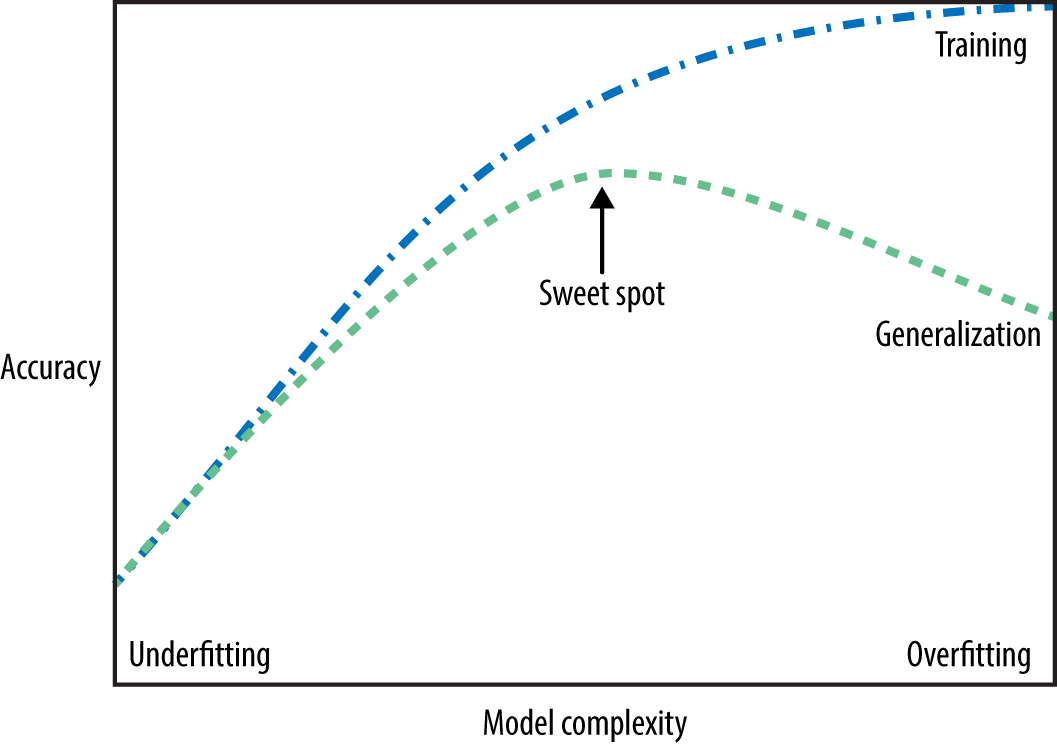
\includegraphics[scale = 0.35]{images/sweet_spot.png}
    \caption{Compromesso tra precisione nella predizione e complessità del modello \cite{figure_copyright}. Nell'asse delle ascisse è rappresentata la complessità del modello, mentre nell'asse delle ordinate la precisione nella predizione dei dati. La curva blu rappresenta la predizione sul training set, che tende ad essere più precisa più il modello è complesso. La curva verde rappresenta la predizione su nuovi set di dati, che come possiamo vedere tende a essere meno precisa quando il modello è troppo complesso e si adatta in maniera eccessiva al training set.}
    \label{fig:sweet_spot}

\end{figure}


\bigskip
I paragrafi che seguono descrivono nello specifico alcuni algoritmi di apprendimento supervisionato.

\subsubsection{k-Nearest Neighbor}

Il \textit{k-Nearest Neighbor} è un algoritmo utilizzato sia in problemi di classificazione sia in problemi di regressione. 
Questo algoritmo si basa sugli attributi degli oggetti del training set che sono vicini a quello che vogliamo classificare, utilizzando un'opportuna distanza. Viene utilizzato un \textit{k} fissato, che indica il numero di vicini da prendere in considerazione per fare la predizione.

Supponiamo di avere due  caratteristiche, che chiameremo $C_{0}$ e $C_{1}$, le quali descriveranno, insieme alla classe, ogni oggetto del nostro dataset. Nel caso di classificazione tramite k-Nearest Neighbor, in Figura \ref{fig:knearest_3_vicini} è mostrato come un elemento ancora non etichettato venga classificato in base al tipo predominante dei suoi vicini.


\begin{figure}[ht]
    \centering
    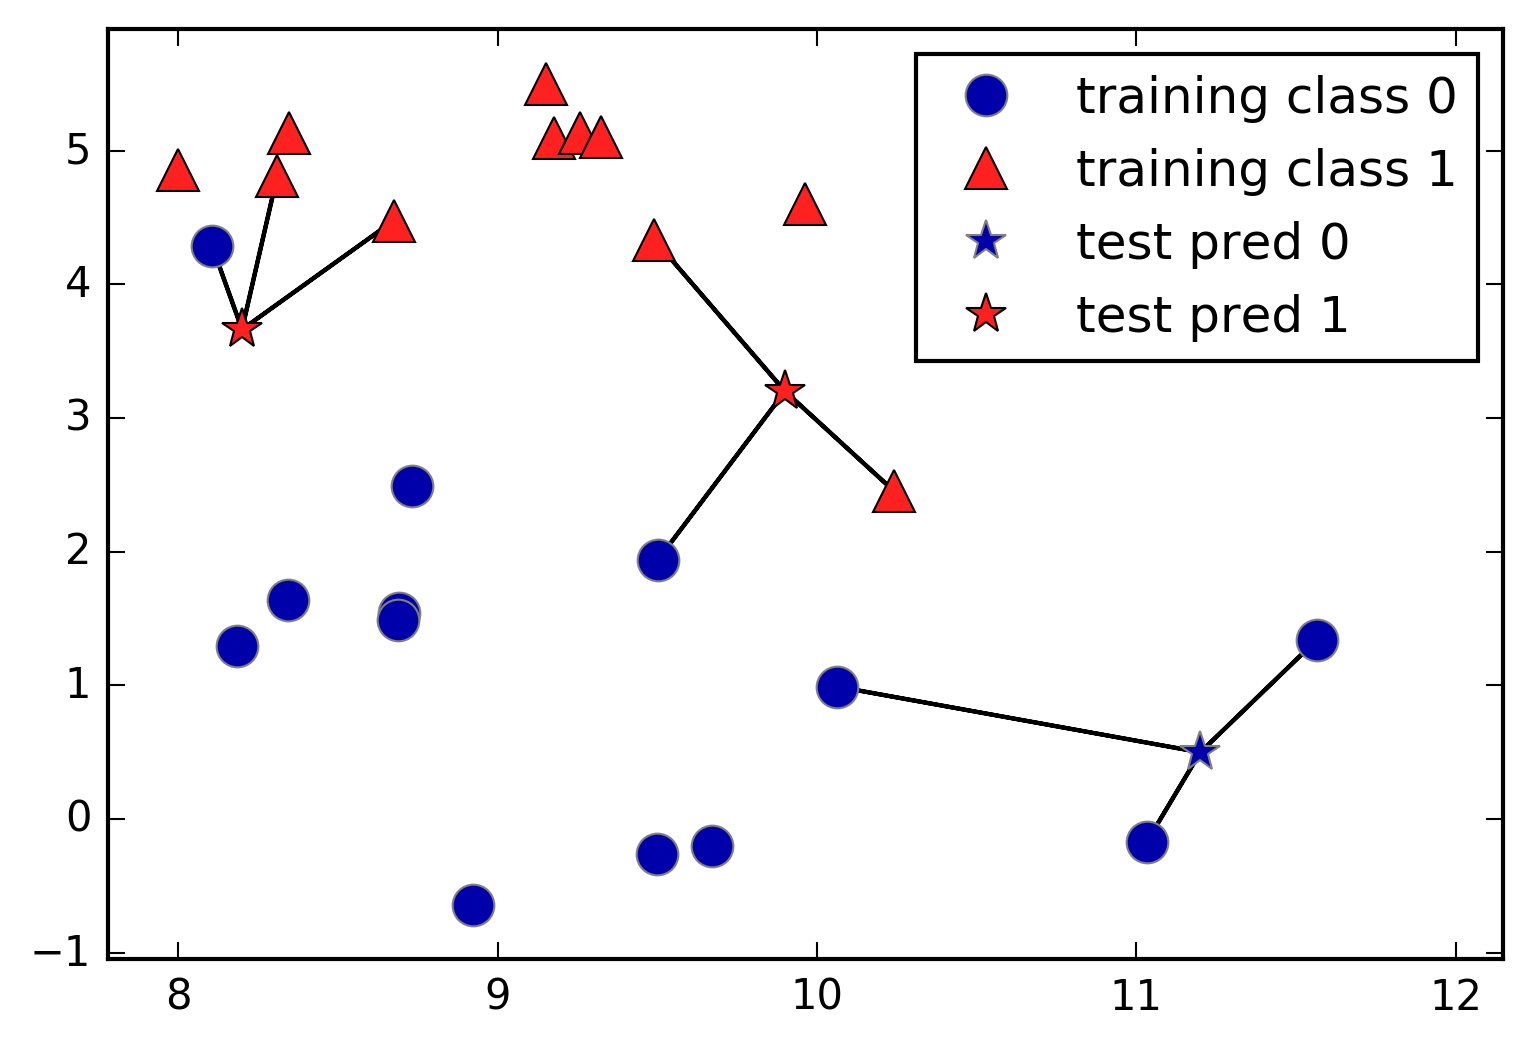
\includegraphics[scale = 0.2]{images/knearest_3_vicini.png}
    \caption{Classificazione tramite k-Nearest Neighbor di 3 elementi. Le stelle rosse rappresentano una classificazione rispetto alla classe 1 (dei triangoli) mentre le stelle blu rappresentano una classificazione rispetto alla classe 0 (dei cerchi) \cite{figure_copyright}.}
    \label{fig:knearest_3_vicini}
\end{figure}

La scelta di \textit{k} dipende dalle caratteristiche dei dati. Generalmente all'aumentare di \textit{k} si riduce il rumore che compromette la classificazione, ma il criterio di scelta per la classe diventa più labile.
Questo algoritmo sceglie la classe che occorre maggiormente nei \textit{k} vicini. Infatti nel caso della classificazione binaria è meglio scegliere un \textit{k} dispari per escludere casi di indecisione e quindi poter sempre definire la classe del nuovo dato. In Figura \ref{fig:differenza_vicini} viene mostrato come influisce la scelta di differenti parametri \textit{k} su uno stesso campione.

\begin{figure}[ht]
    \centering
    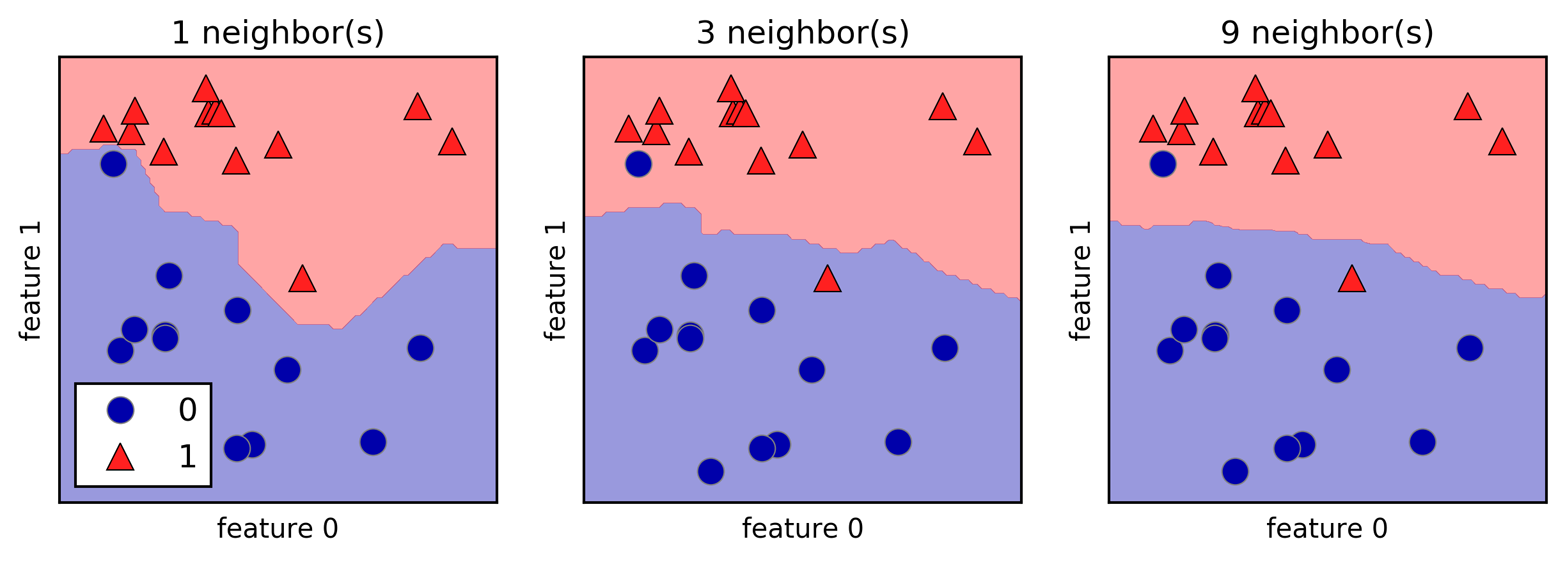
\includegraphics[scale = 0.2]{images/knearest_differenza_vicini.png}
    \caption{Risultati di un classificatore k-Nearest Neighbor, per diversi valori del parametro \textit{k} su un medesimo dataset. I cerchi e i triangoli indicano le osservazioni del dataset appartenenti a due classi, mentre le aree blu e rosse indicano gli esiti della classificazione \cite{figure_copyright}.}
    \label{fig:differenza_vicini}
\end{figure}

Nel caso di regressione il ragionamento alla base è molto simile. Immaginiamo di avere un dataset con due caratteristiche per ogni oggetto: \textit{Target}, il valore che vogliamo predire, e \textit{Feature}, il valore su cui vogliamo basare il modello. Prendendo \textit{k} pari a 3 otteniamo, come mostrato in Figura \ref{fig:knearest_regression}, che il nuovo elemento da predire avrà come valore \textit{Target} la media dei 3 elementi più vicini sull'asse delle \textit{Feature}.

\begin{figure}[h]
    \centering
    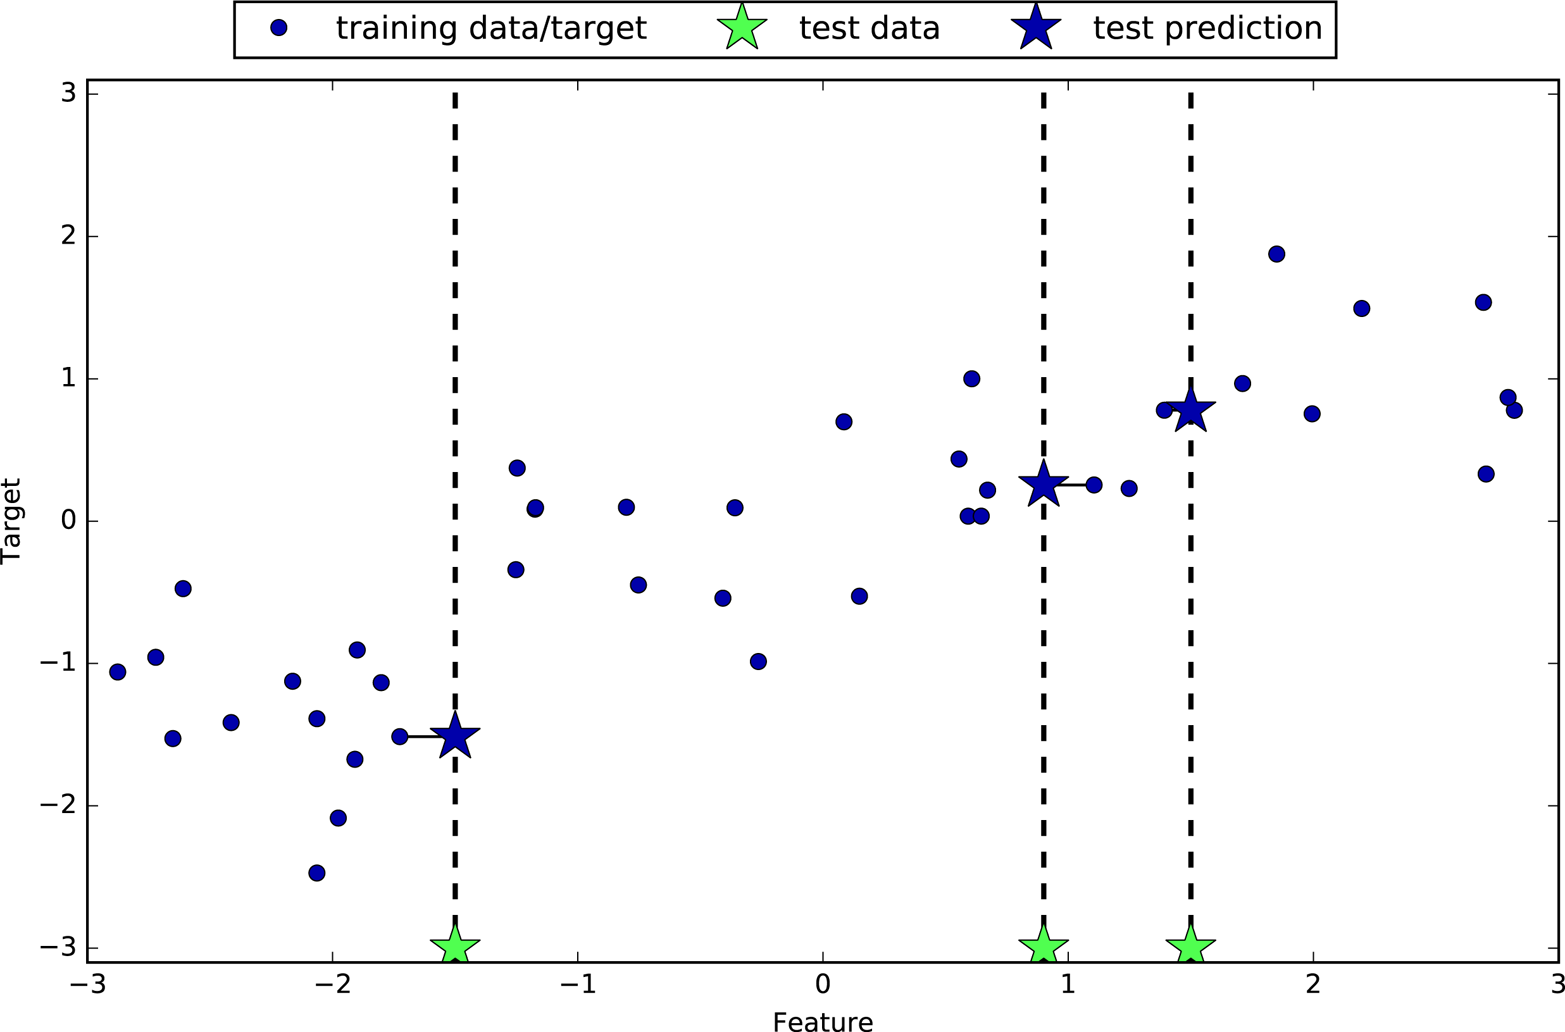
\includegraphics[scale = 0.19]{images/knearese_regression_3k.png}
    \caption{Risultato di un regressore k-Nearest Neighbor con \textit{k} pari a 3. I cerchi rappresentano gli oggetti del dataset, le stelle verdi indicano il nuovo elemento da predire mentre le stelle blu rappresentano gli esiti delle predizioni \cite{figure_copyright}.}
    \label{fig:knearest_regression}
\end{figure}

Un'altra scelta importante da considerare quando utilizziamo questo algoritmo è come calcolare la distanza dei vicini, ovvero secondo quale criterio scegliere i vicini. Finora abbiamo considerato una distanza euclidea, ma a seconda del contesto trattato è opportuno scegliere una metrica adatta \cite{distance_metrics_knn}. 

\subsubsection{Modelli lineari}
I modelli lineari cercano di effettuare predizioni utilizzando una funzione lineare basata sull'insieme delle caratteristiche dell'elemento da analizzare.

Nel caso della regressione, la funzione è definita come segue: 

\begin{equation*}
    y  = w_0x_0 + w_1x_1 + \dots + w_nx_n + b
\end{equation*}

\noindent dove \textit{n} è il numero di caratteristiche, $x_i$ sono le caratteristiche, $w_i$ i pesi da attribuire a esse, e $b$ un termine noto.
Il valore $y$ ottenuto applicando la funzione lineare alle caratteristiche di un particolare caso rappresenta la predzione per l'etichetta corrispondente.

Riprendendo l'esempio precedente, supponiamo di voler quantificare il numero di giorni necessari per guarire un paziente malato. Per semplicità supponiamo di avere come unica caratteristica l'età del paziente. In Figura \ref{fig:linear_regression} è rappresentato il dataset dei pazienti. \`E possibile tracciare una retta denominata \textit{retta di regressione} che approssima tutti i punti nel dataset.

\begin{figure}[h]
    \centering
    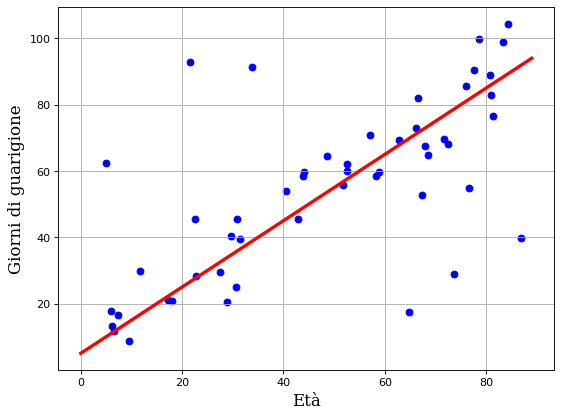
\includegraphics[scale=0.7]{images/regressione_lineare.png}
    \caption{Regressione lineare. Nell'asse delle ascisse indichiamo l'età dei pazienti, mentre in quello delle ordinate indichiamo i giorni necessari per la guarigione. I punti in blu rappresentano i pazienti nel dataset, mentre la retta rossa rappresenta la retta di regressione che approssima meglio l'andamento di tutti i punti.}
    \label{fig:linear_regression}

\end{figure}


I modelli lineari si possono applicare anche al contesto della classificazione, introducendo degli intervalli sui valori di $y$ per definire a quale classe appartiene il singolo caso. 
Per la classificazione binaria, immaginando di avere due classi, $C_1$ e $C_0$, potremmo avere una formula che associa l'oggetto alla classe $C_0$ se

\begin{equation*}
    y = w_0x_0 + w_1x_1 + \dots + w_nx_n + b > 0
\end{equation*}

\noindent e alla classe $C_1$ altrimenti.


\subsubsection{Alberi di decisione}

Un albero di decisione (\textit{Decision Tree}) è un modello predittivo utilizzato sia per la classificazione che per la regressione, la cui logica si basa su una struttura ad albero.In quest'ultimo ogni nodo interno rappresenta un controllo su una variabile; ogni foglia corrisponde  alla classe o etichetta che rappresenta la predizione per l'oggetto di partenza.
I controlli sulle variabili sono spesso di tipo binario.

\begin{figure}[h]
    \centering
    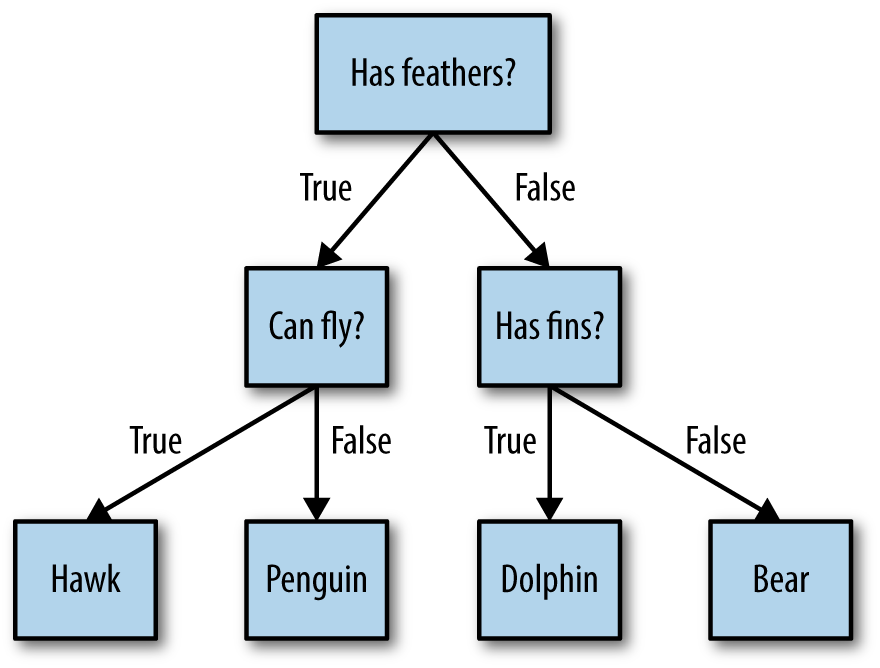
\includegraphics[scale=0.35]{images/decisione_tree.png}
    \caption{Esempio di albero di decisione per la classificazione di un animale \cite{figure_copyright}.}
    \label{fig:decision_tree}

\end{figure}

Ad esempio supponiamo di voler distinguere un animale tra: falco, pinguino, delfino e orso. Nell'esempio in Figura \ref{fig:decision_tree} l'algoritmo parte dalla domanda ``Ha le piume?''. In questo modo abbiamo definito il primo nodo dell'albero. Sapendo che, in questo caso, i test previsti restituiscono un output binario, da questo primo nodo si diramano due sotto-alberi rapprensentati dalle categorie ``Ha le piume'' e ``Non ha le piume''. Mediante un'ulteriore domanda si possono distinguere gli animali. Per esempio seguendo la domanda ``Può volare?'', se la risposta è sì, si sta parlando del falco, ovvero l'unico animale tra i quattro che ha le piume e che può volare, altrimenti si tratta del pinguino. Seguendo questa logica è posssibile arrivare a fare delle predizioni. 
L'esempio è chiaramente fittizio. Nella realtà i dati che vengono analizzati hanno spesso valori di tipo continuo, con test come ``\textit{x} è minore di \textit{k}?'', dove \textit{x} è la caratteristica considerata e \textit{k} una costante.

I problemi di \textit{overfitting} e \textit{underfitting} sono problemi ricorrenti che si presentano anche nel caso degli alberi di decisione. Infatti se viene costruito un albero troppo dettagliato, e quindi con un elevato livello di profondità, il modello tende ad adattarsi in maniera eccessiva ai dati usati in fase di allenamento generando un problema di \textit{overfitting}.
Aumentando la profondità dell'albero, infatti, l'errore su un insieme di dati non incluso in quello di allenamento cresce.

Più permettiamo all’albero di avere tanti livelli, più questo ha la capacità di adattarsi meglio ai dati di training, e a partire da una certa lunghezza inizia a farlo a detrimento della sua capacità di generalizzazione. 

Per risolvere questo problema esistono due strategie:
\begin{itemize}
    \item limitare a priori la profondità dell'albero, 
    \item eliminare i nodi che contengono informazioni poco significative.
\end{itemize}

% \begin{figure}[ht]
%     \centering
%     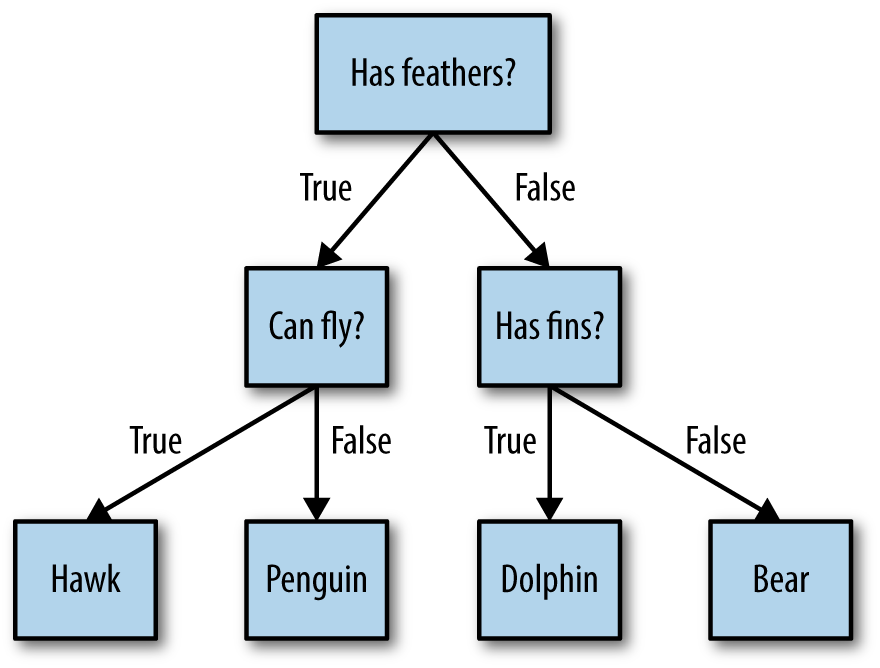
\includegraphics[scale = 0.3]{images/decisione_tree.png}
%     \label{fig:decision_tree}
%     \caption{Esempio di albero di decisione per la classificazione di un animale. \cite{figure_copyright}}
% \end{figure}

\subsubsection{Support Vector Machine}
Le \textit{Support Vector Machine} sono dei modelli di apprendimento utilizzati sia per la regressione che la classificazione.
Una \textit{Support Vector Machine} \cite{SVM} per la classificazione individua un iperpiano o un insieme di iperpiani per separare i punti in uno spazio e quindi dividerli in diversi gruppi.

Supponiamo di avere un dataset con oggetti appartenenti a due classi, come in Figura \ref{fig:svm}, e di voler trovare un iperpiano che divide le due classi. Come possiamo vedere nella Figura 12(\ref{sub@fig:iperpiani_svm}) ci sono molti possibili iperpiani che dividono le due classi. Il nostro obiettivo è quello di trovare il piano che ha il margine massimo, ovvero quel piano che massimizza la distanza da entrambe le classi, come in Figura 12(\ref{sub@fig:iperpiano_ideale}). I punti del dataset più vicini all'iperpiano e che influenzano la sua posizione vengono chiamati \textit{vettori di supporto} (\textit{Support Vector}, da qui il nome dell'algoritmo). Eliminare uno di questi punti cambierebbe la posizione dell'iperpiano, Per questo motivo, possono essere considerati gli elementi critici di un set di dati.

\begin{figure}[ht]
    \begin{subfigure}{0.47\textwidth}
        \centering
        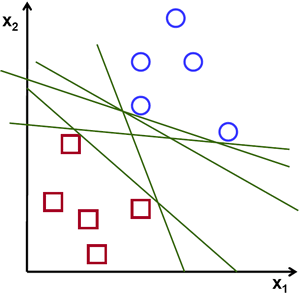
\includegraphics[scale=0.5]{images/iperpiani_svm.png}
        \caption{Iperpiani possibili.}
        \label{fig:iperpiani_svm}
    \end{subfigure}
    \begin{subfigure}{0.47\textwidth}
        \centering
        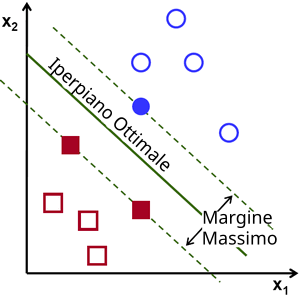
\includegraphics[scale=0.5]{images/iperpiano_ottimale_svm_ita.png}
        \caption{Iperpiano ideale.}
        \label{fig:iperpiano_ideale}
    \end{subfigure}
    \caption{Scelta dell'iperpiano ideale. In questo caso vengono mostrate due classi, i quadrati rossi e i cerchi blu, in un piano bidimensionale, quindi l'iperpiano che dividerà le due classi sarà una retta. Nella Figura (\protect\subref{fig:iperpiani_svm}) vengono mostrati alcuni possibili iperpiani che dividono le due classi. Mentre nella Figura (\protect\subref{fig:iperpiano_ideale}) viene mostrato l'iperpiano ideale con il massimo margine dalle due classi. Inoltre gli oggetti colorati rappresentano i vettori di supporto \cite{SVM}. }
    \label{fig:svm}
\end{figure}

Spesso succede che le classi da distinguere non siano linearmente separabili nello spazio in cui è definito il problema originale. Per risolvere questo problema si ricorre alle funzioni \textit{kernel} che sono in grado di mappare dei vettori dallo spazio originale ad uno spazio a dimensionalità più elevata, in cui le immagini risultano linearmente separabili.

\subsection*{Approccio Non Supervisionato}
Con \textit{Approccio Non Supervisionato} \cite{unsupervised_learning} ci riferiamo a una tecnica di apprendimento automatico che consiste nel fornire in input una serie di dati non etichettati ma che verranno raggruppati sulla base di caratteristiche comuni  per cercare di effettuare delle previsioni su input futuri.
% L'apprendimento non supervisionato è una tecnica di apprendimento automatico che consiste nel fornire alla macchina una serie di input che verranno riclassificati e organizzati sulla base di caratteristiche comuni per cercare di effettuare ragionamenti e previsioni sugli input successivi.
Al contrario dell'apprendimento supervisionato, durante l'apprendimento vengono forniti solo esempi non annotati, in quanto le classi non sono note a priori ma devono essere apprese automaticamente.

\bigskip

La principale tecnica in questa categoria è il \textit{clustering}, ovvero una tecnica in grado di suddividere in gruppi distinti  gli oggetti presi in considerazione.
Un esempio di utilizzo ricade nell'ambito della sicurezza informatica. Gli attacchi effettivamente rilevati sono probabilmente solo la punta dell'iceberg. Utilizzando tecniche di clustering è possibile individuare e bloccare attacchi ancora sconosciuti.

Il Machine Learning non supervisionato potrebbe utilizzare informazioni dei clienti sugli utilizzi abituali dei servizi di una banca. Se un malintenzionato provasse a effettuare delle operazioni tramite il nostro conto bancario dall'altra parte del mondo a un orario differente da quello abituale, l'uso di tecniche di clustering permette di riconoscere le operazioni abituali e mandare un messaggio di allarme se vengono individuati casi anomali.

\subsection*{Approccio Semi-Supervisionato}
A metà strada tra l'apprendimento supervisionato e quello non supervisionato c'è l'apprendimento \textit{Semi-Supervisionato} \cite{supervisedlearning}.

Questo approccio consiste nel combinare le due tecniche descritte nei paragrafi precedenti e fornire un risultato basandosi su un input eterogeneo costituito da dati etichettati e dati non etichettati.
Questo perché le etichette dei dati a volte possono essere difficili da reperire, costosi e dispendiosi in termini di tempo e di denaro da recuperare, dato che spesso i dati vengono etichettati manualmente da utenti specializzati. Allo stesso tempo i dati non etichettati possono essere relativamente facili da raccogliere, ma ci sono pochi modi di utilizzarli. 
L'approccio semi-supervisionato risolve questi problemi utilizzando una grande quantità di dati non etichettati, insieme a una porzione di dati etichettati, per costruire classificatori migliori. 

Ma com'è possibile, avendo a confronto l'apprendimento supervisionato che utilizza solo dati etichettati, avere classificatori migliori tenendo in considerazione i dati non etichettati?
Utilizzando una metafora matematica \cite{supervisedlearning}, potremmo dire che la conoscenza di $p(x)$ che acquisiamo attraverso i dati non etichettati è un'informazione utile per la predizione di $p(y|x)$. Se non fosse questo il caso, allora non avremo alcun vantaggio rispetto l'apprendimento supervisionato.

\subsection*{Apprendimento con rinforzo}
%%
Il quarto e ultimo approccio, chiamato \textit{Approccio con rinforzo} \cite{Reinforcement_learning}, ha come finalità quella di costruire degli agenti autonomi che hanno il compito di scegliere le azioni da compiere per conseguire determinati scopi attraverso lo studio e l'interazione con il sistema circostante.
In sostanza, utilizzando questo approccio, non siamo noi che istruiamo la macchina, bensì questa decide le azioni da compiere a seconda dello stato attuale del sistema, e così facendo ne determina quello futuro.
%%

Quando la macchina prende una decisione otterrà successivamente una “ricompensa”, sotto forma di punteggio, che sarà alto se la decisione presa è giusta o basso altrimenti. Così l'agente cercherà di fare sempre meglio per arrivare a ottenere il punteggio più alto possibile, prendendo decisioni corrette.

% Link tra insiemi fuzzy e machine learning.
\chapter{Tecnologie e metodologie}
\label{Capitolo 2}
\section{\texorpdfstring{$\mu$}{mu}-learn}
Nel capitolo precedente abbiamo visto alcune tecniche utilizzate nel Machine Learning. L’algoritmo che andremo a descrivere, denominato \textit{$\mu$-learn} e descritto nel dettaglio in \cite{mulearn}, si basa sull’ induzione di insiemi fuzzy e ricade nell’approccio supervisionato, ovvero quella tecnica che necessita di dati preventivamente valutati per effettuare predizioni. In questo caso la predizione è il grado di appartenenza.
\bigskip

Supponiamo di avere un campione $X = \{x_1,\dots,x_m\}$, e un insieme di gradi di appartenenza $ M = \{\mu_1,\dots,\mu_m\}$ associati a un generico insieme fuzzy $A$. L'obiettivo di \textit{$\mu$-learn} consiste nel determinare un'approssimazione di $A$ partendo dai valori contenuti in $X$ e $M$.
Il problema di apprendere $\mu_A$ può essere suddiviso in due parti:
\begin{itemize}
    \item determinare la forma di A;
    \item indurre i parametri della funzione di membership $\mu_A$.
\end{itemize}

\noindent Per fare ciò dobbiamo partire dalle seguenti ipotesi:
\begin{itemize}
    \item  Definiamo il \textit{core} di $A$ come l'insieme di tutti gli elementi dell'universo in corrispondenza dei quali il grado di appartenenza di $A$ è uguale a 1:
    \begin{equation*}
        A_C = \{ x\in U \hspace{0,3cm} |\hspace{0,3cm} \mu_A(x) = 1 \}
    \end{equation*}
    \noindent Il core di $A$ si può approssimare come l'insieme degli elementi di $U$ le cui immagini mappate tramite una funzione $\Phi: U \to V$ sono incluse in un'ipersfera di centro $a$ e raggio $R$.

    \item Il grado di appartenenza $\mu_A(x)$ dipende solo dalla distanza tra $\Phi(x)$ e $a$.
\end{itemize}

\noindent Fatte queste ipotesi è possibile definire il problema: trovare la più piccola sfera avente centro $a$ e raggio $R$ che includa la maggior parte delle immagini mappate tramite $\Phi$ degli elementi $x\in X$ che hanno un grado di appartenenza alto ed escludere le immagini rimanenti.



La formulazione matematica di questo problema determina un problema di ottimizzazione vincolata, la cui funzione obiettivo è:
\begin{equation}
    \min R^2 + C\displaystyle\sum_{i=1}^{n}(\xi_i+\tau_i)
    \label{eq:Problema_di_partenza}
\end{equation}
sottoposta ai seguenti vincoli:
\begin{equation}
    \mu_i\|\Phi(x_i)-a\|^2\le\mu_iR^2 + \xi_i,
    \label{eq:vincolo_1}
\end{equation}
\begin{equation}
    (1-\mu_i)\|\Phi(x_i)-a\|^2 \ge (1-\mu_i)R^2 - \tau_i,
    \label{eq:vincolo_2}
\end{equation}
\begin{equation}
    \xi_i \ge 0, \tau_i \ge 0,
    \label{eq:vincolo_3}
\end{equation}


\noindent dove $\xi$ e $\tau$ sono le variabili di scarto utilizzate nel problema di ottimizzazione. $\xi$ è la variabile slack legata al posizionamento dei punti all'interno della sfera, mentre $\tau$ è riferita al posizionamento dei punti all'esterno della sfera. Infine $C$ è una costante la cui funzione è quella di `pesare' l'impatto delle variabili di slack.

Possiamo notare che quando $\mu_i = 1$ il vincolo (\ref{eq:vincolo_1}) diventa:
\begin{equation*}
    \|\Phi(x_i)-a\|^{2} \le R^2 + \xi_i,
\end{equation*}
ovvero che la distanza della trasformazione di $x_i$ da $a$ deve possibilmente essere minore o uguale al raggio della sfera e che il vincolo (\ref{eq:vincolo_2}) diventa:
\begin{equation*}
    \tau_i \ge 0,
\end{equation*}
che è già incorporato nel vincolo (\ref{eq:vincolo_3}), e quindi l'ottimizzazione tenderà a posizionare l'immagine all'interno della sfera.

Allo stesso modo, quando $\mu_i = 0$ il vincolo (\ref{eq:vincolo_2}) diventa:
\begin{equation*}
    \|\Phi(x_i)-a\|^2 \ge R^2 - \tau_i,
\end{equation*}
ovvero che la distanza della trasformazione di $x_i$ da $a$ è maggiore o uguale al raggio della sfera e il vincolo (\ref{eq:vincolo_1}) diventa:
\begin{equation*}
    \xi_i \ge 0,
\end{equation*}
che è già incorporato nel vincolo (\ref{eq:vincolo_3}), e quindi il nostro $x_i$ sarà posizionato all'esterno della sfera.

Utilizzando la formulazione duale di Wolfe, quello che otteniamo è il seguente problema:
\begin{equation}
\begin{split}
    \max \displaystyle\sum_{i=1}^{m}(\alpha_i\mu_i - \beta_i(1-\mu_i))&k(x_i,x_i)\hspace{0,1cm}- \\ &\displaystyle\sum_{i,j=1}^{m}(\alpha_i\mu_i - \beta_i(1-\mu_i))(\alpha_j\mu_j - \beta_j(1-\mu_j))k(x_i,x_j)
\end{split}
\label{eq:problema_finale}
\end{equation}
sottoposto ai vincoli:
\begin{equation}
    \displaystyle\sum_{i=1}^{n}(\alpha_i\mu_i - \beta_i(1-\mu_i)) = 1,
    \label{eq:v1_problema_finale}
\end{equation}
\begin{equation}
    0 \le \alpha_i,\beta_i \le C,
    \label{eq:v2_problema_finale}
\end{equation}

\noindent dove $k$ è la funzione kernel associata alla mappatura nello spazio dell'immagine di $\Phi$ (ovvero $k(x_i,x_j) = \Phi(x_i)\cdot\Phi(x_j))$.

Indicando con $^*$ il valore ottimale per una variabile, è possibile dimostrare che per ogni $x$ nel corrispondente dominio vale la seguente proprietà:
\begin{equation*}
\begin{split}
    R^{2}(x) = k(x,x) \hspace{0,1cm}- \hspace{0,1cm}&2\displaystyle\sum_{i=1}^{m}(\alpha_{i}^{*}\mu_{i} - \beta_{i}^{*}(1-\mu_{i}))k(x,x_i)\hspace{0,1cm} + \\ 
    &\displaystyle\sum_{i,j=1}^{m}(\alpha_{i}^{*} - \beta_{i}^{*}(1-\mu_{i}))(\alpha_{j}^{*} - \beta_{j}^{*}(1-\mu_{j}))k(x_i,x_j).
\end{split}
\end{equation*}

\noindent Così facendo è possibile calcolare la distanza tra il centro della sfera e l'immagine del punto dato $x$.
In particolare, la maggior parte dei punti $x$ con un valore di membership $\mu_{A}(x) > \frac{1}{2}$ soddisfanno $R^2(x) \le R^2_1$ dove $R^2_1 = R^2(x_i)$ per qualunque vettore di supporto.
Apprendere la funzione di membership richiede di trovare il giusto compromesso nella scelta del parametro $C$, così come nei parametri del kernel.

\subsection*{Configurazione degli Iperparametri}
Nel contensto del Machine Learning si parla spesso di iperparametri. Si definiscono iperparametri quei parametri utilizzati per aver un certo tipo di controllo sul processo di apprendimento. In altre parole, tutti i dati forniti dall'utente che influiscono sul design del modello sono considerati iperparametri. Un primo parametro da considerare è quello della scelta della funzione di kernel.
Esistono diversi tipi di funzioni di kernel.

\begin{itemize}
    \item \textbf{Kernel Lineare}. \`E uno dei più semplici e consiste nel prodotto scalare di due vettori:
    \begin{equation*}
        k(x,y) = x \cdot y.
    \end{equation*}

    \item  \textbf{Kernel Polinomiale}. Viene utilizzato per gestire problemi di suddivisione non lineare ed è definito come segue:
    \begin{equation*}
        k(x,y) = (x \cdot y + c)^{d},
    \end{equation*}
    \noindent dove $c$ è  una costante e $d$ indica il grado del polinomio.

    \item \textbf{Kernel Gaussiano}. Utilizzato per scopi più generici, è rappresentato da:
    \begin{equation*}
        k(x,y) = \exp{\bigg(-\frac{\|x-y\|^{2}}{2\sigma^{2}}\bigg)},
    \end{equation*}
    \noindent dove $\sigma$ è la deviazione standard del kernel. Dato che questo è il kernel utilizzato durante gli esperimenti descritti nel Capitolo \ref{Captiolo 3}, $\sigma$ diventa un parametro chiave da considerare. Prendendo l'esemprio in Figura \ref{fig:parametro_sigma} e una funzione kernel, vediamo come la scelta del parametro $\sigma$ modifichi la forma della funzione di appartenenza. La funzione tratteggiata rappresenta una funzione di apparteneza fissata, dove sull'asse delle ascisse ci sono i valori di $x$, colorati in funzione del valore associato a questa funzione. La curva blu invece rappresenta la funzione di appartenenza appresa a partire dai punti.

    \begin{figure}[h]
        \begin{subfigure}[t]{0.32\textwidth}
           \centering
           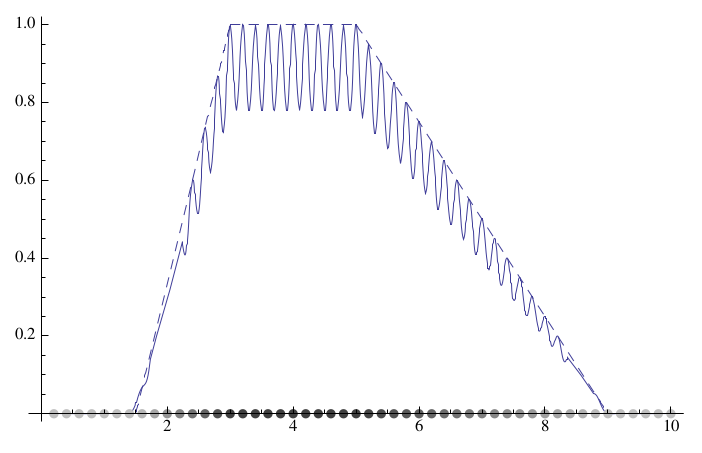
\includegraphics[scale=0.18]{images/parametro_sigma_1.png}
           \caption{$\sigma = 0.075 $}
           \label{fig:sigma_1}
    
        \end{subfigure}
        \begin{subfigure}[t]{0.32\textwidth}
            \centering
            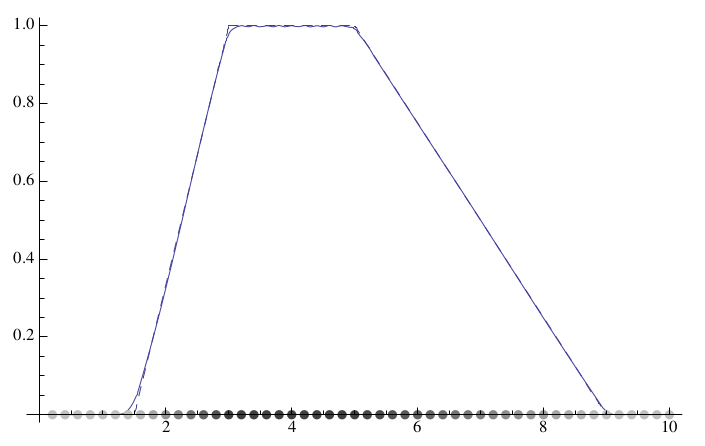
\includegraphics[scale=0.18]{images/parametro_sigma_2.png} 
            \caption{$\sigma = 0.12 $}
            \label{fig:sigma_2}
    
        \end{subfigure}
        \begin{subfigure}[t]{0.32\textwidth}
            \centering
            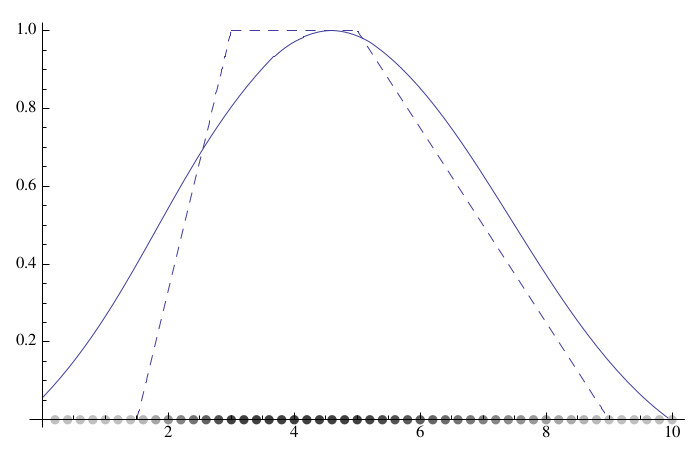
\includegraphics[scale=0.18]{images/parametro_sigma_3.png}
            \caption{$\sigma = 2 $}
            \label{fig:sigma_3}
        \end{subfigure}
        \caption{Nelle figure possiamo vedere come al variare del parametro $\sigma$ la forma della funzione di appartenenza cambi. In particolare all'aumentare di $\sigma$ notiamo come la forma della funzione sia più smussata.}
        \label{fig:parametro_sigma}
    \end{figure}

    \item  \textbf{Kernel Iperbolico}. Prende il nome da una delle funzioni di attivazione utilizzate nelle reti neurali ed è definito come:
    \begin{equation*}
        k(x,y) = \tanh (\alpha x\cdot y + \beta),
    \end{equation*}
    \noindent dove $\alpha$ e $\beta$ sono rispettivamente il fattore di scala e l'offset.
\end{itemize}


\noindent Un secondo parametro da considerare è la constante $C$ che compare nella funzione obiettivo (\ref{eq:Problema_di_partenza}). Questa ha lo scopo di definire il costo dell'errore nella classificazione degli elementi durante la costruzione dell'ipersfera. Più $C$ è grande, più sarà elevato il costo dell'errore nel posizionamento delle immagini dei punti dentro o fuori l'ipersfera. Viceversa, più $C$ è piccola , più il costo dell'errore diminuisce. In Figura \ref{fig:parametro_C} vediamo come un determinato valore di $C$ ci permette di avere un errore quasi nullo (possiamo notare come nel grafico 14(\subref{fig:C_1}) la funzione di appartenenza appresa a partire dai punti si sovrappone quasi perfettamente con la funzione di apparteneza fissata), e all'aumentare di $C$ la funzione tende a diventare binaria.

\begin{figure}[h]
    \begin{subfigure}[t]{0.32\textwidth}
       \centering
       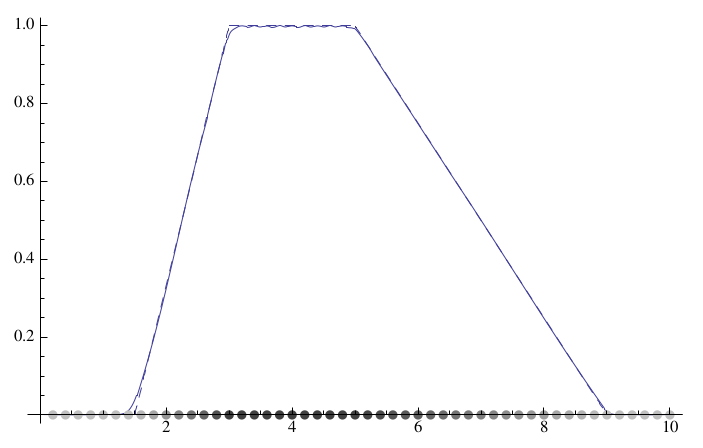
\includegraphics[scale=0.18]{images/parametro_C_1.png}
       \caption{$C = 0.0421 $}
       \label{fig:C_1}

    \end{subfigure}
    \begin{subfigure}[t]{0.32\textwidth}
        \centering
        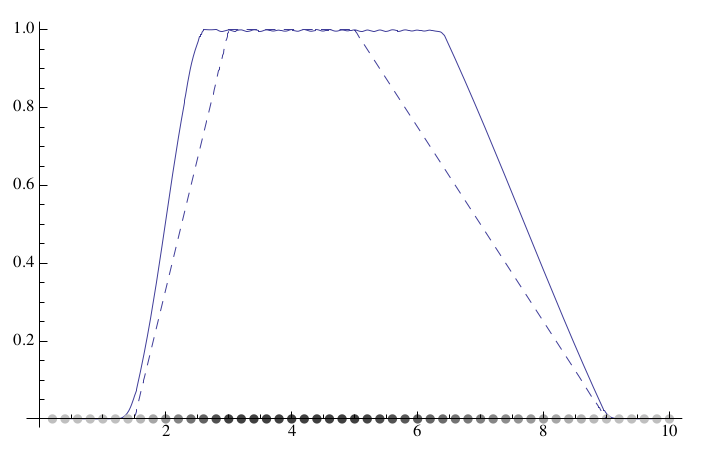
\includegraphics[scale=0.18]{images/parametro_C_2.png} 
        \caption{$C = 0.08 $}
        \label{fig:C_2}

    \end{subfigure}
    \begin{subfigure}[t]{0.32\textwidth}
        \centering
        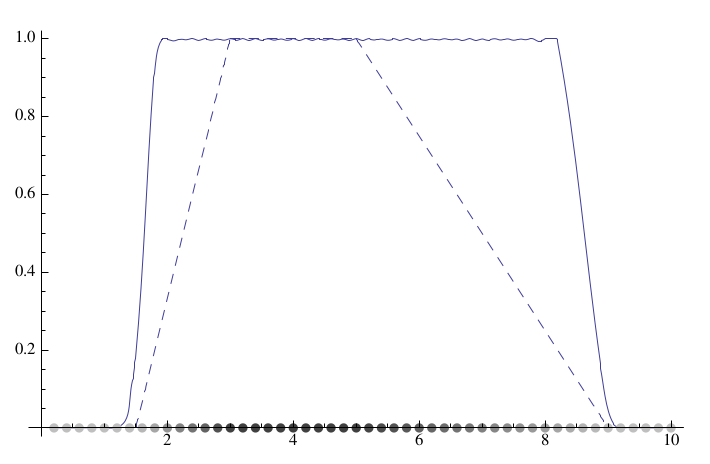
\includegraphics[scale=0.18]{images/parametro_C_3.png}
        \caption{$C = 0.15 $}
        \label{fig:C_3}
    \end{subfigure}
    \caption{Nelle figure è mostrato come all'aumentare di $C$ la funzione di appartenenza appresa tenda ad aumentare la sua larghezza, avvicinandosi sempre di più ad una funzione di appartenenza binaria.}
    \label{fig:parametro_C}
\end{figure}

%ESEMPI DI KERNEL E I VARI PARAMETRI

\section{Descrizione del problema}
Nel paragrafo precendete abbiamo descritto un problema di ottimizzazione vincolata. In questo paragrafo vedremo com'è possibile costruirne un'implementazione per la risoluzione.

\bigskip

\noindent Ponendo $\chi_i = (\alpha_i\mu_i - \beta_i(1-\mu_i))$, il problema \ref{eq:problema_finale} può essere riscritto come:
\begin{equation}
    \max \displaystyle\sum_{i=1}^{n}\chi_ik(x_ix_i) -\displaystyle\sum_{i,j=1}^{n}\chi_i\chi_j k(x_i,x_j),
\label{eq:problema_finale_2}
\end{equation}

\noindent mentre i vincoli (\ref{eq:v1_problema_finale}) (\ref{eq:v2_problema_finale}) diventano:

\begin{equation}
    \displaystyle\sum_{i=1}^{n}\chi_i = 1,
    \label{eq:v1_problema_finale_2}
\end{equation}
\begin{equation}
    -C(1-\mu_i) \le \chi_i \le C\mu_i.
    \label{eq:v2_problema_finale_2}
\end{equation}

\noindent Come possiamo vedere, grazie a questa manipolazione matematica, quello che otteniamo è un problema di ottimizzazione convessa quadratico vincolato.
Nell'ambito della risoluzione di questo tipo di problema in Python ci sono a disposizione diversi software che permettono di modellare e risolvere il problema.

In particolare la risoluzione di questo problema viene implementata nella parte di ottimizzazione dell'algoritmo \textit{$\mu$-learn} \cite{mulearn_documentation}. Il modulo \textit{optimization} contiente l'implementazione di uno \textit{Strategy pattern} \cite{strategy_pattern}. Come mostrato nel diagramma UML in Figura \ref{fig:diagramma_uml}, la classe \textit{Solver} è l'interfaccia astratta che implementa il metodo \textit{solve}, il quale delega il processo di ottimizzazione al metodo astratto \textit{solve\_problem}, che viene implementato concretamente nelle diverse classi risolutrici.

\begin{figure}
    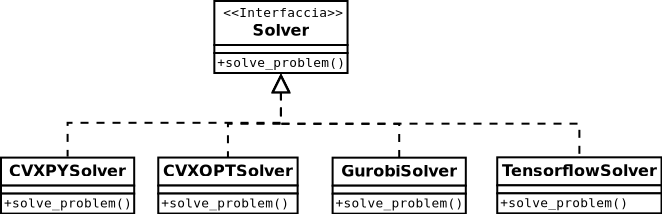
\includegraphics[scale=0.6]{images/diagramma_uml.png}
    \centering
    \caption{Diagramma UML dello Strategy pattern implementato nel modulo di ottimizzazione dell'algoritmo $\mu$-learn.}
    \label{fig:diagramma_uml}
\end{figure}

I parametri necessari per implementare il metodo \textit{solve} sono i seguenti: 
\begin{itemize}
    \item \textbf{xs}: gli oggetti del training set;
    \item \textbf{mus}: i valori di membership per gli oggetti del training set;
    \item \textbf{c}: la costante che pesa l'impatto delle variabili di slack sul problema;
    \item \textbf{k}: la funzione kernel da utilizzare, scelta tra quelle implementate nel modulo \textit{kernel} della libreria.
\end{itemize}

Di seguito vengono descritti i software con cui sono stati implementati i diversi \textit{Solver}.

\section{CVXOPT}
CVXOPT è un software gratuito utilizzato per l'ottimizzazione convessa basato su Python. Può essere utilizzato tramite un interprete interattivo in Python, attraverso riga di comando eseguendo script in Python, o integrandolo in altre applicazioni per l'ottimizzazione convessa grazie ai moduli di estensione. 
%\cite{CVXOPT}

Il framework di CVXOPT per la risoluzione di problemi di ottimizzazione quadratica vincolata si aspetta il problema formulato secondo la forma standard:
\begin{equation*}
\begin{split}
    \min \hspace{0.2cm}&\frac{1}{2}x^{T}Px + q^{T}x,\\ 
    \textrm{sottoposto a } \hspace{0.2cm} &Gx \preceq h,\\
    &Ax = b.
\end{split}
\end{equation*}

\noindent dove $x^{T}$ denota la trasposta di $x$, e $Gx \preceq h$ indica che la diseguaglianza è applicata elemento per elemento tra i vettori $Gx$ e $h$. 
CVXOPT per risolvere un problema di questo tipo richiede i parametri ${P,q,G,h,A,b}$; dove $P$ e $q$ sono richiesti, gli altri opzionali. Notiamo che il vettore contenente le variabili $x$ non viene passato al solver, ma viene definito implicitamente attraverso i parametri dati, per questo è essenziale che l'ordine delle variabili stesse sia mantenuto per i parametri realtivi (ad esempio $q_i$, $h_i$,$b_i$ devono corrispondere alla variabile $x_i$).

Il nostro problema (\ref{eq:problema_finale_2}) può essere riscritto nel seguente modo per rispettare la forma standard: 
\begin{equation}
    \min \displaystyle\sum_{i,j=1}^{n}\chi_i\chi_j k(x_i,x_j) - \displaystyle\sum_{i=1}^{n}\chi_ik(x_ix_i),
    \label{eq:forma_standard}
\end{equation}
sottoposto ai seguenti vincoli:
\begin{equation}
    \chi_i \le C\mu_i,
    \label{eq:vincolo_1_forma_standard}
\end{equation}
\begin{equation}
    -\chi_i \le C(1-\mu_i),
    \label{eq:vincolo_2_forma_standard}
\end{equation}
\begin{equation}
    \displaystyle\sum_{i=1}^{n}\chi_i = 1.
    \label{eq:vincolo_3_forma_standard}
\end{equation}

\noindent In questo modo è più intuitivo dedurre la forma matriciale:
\begin{figure}[H]
    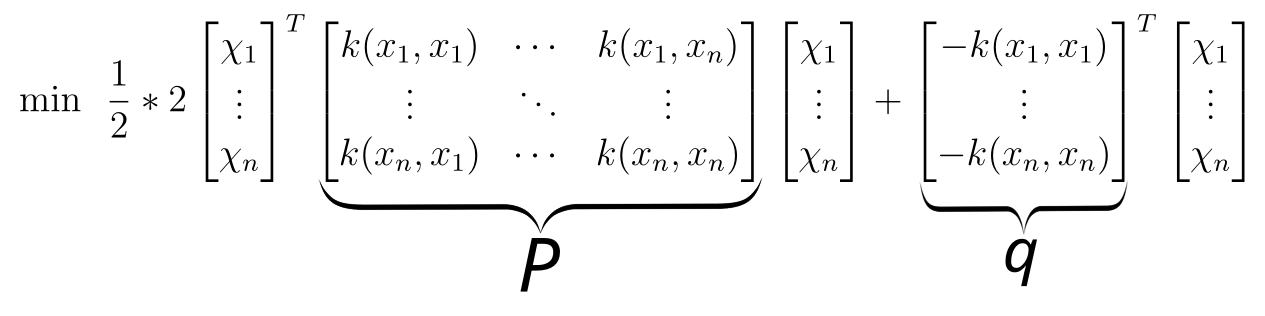
\includegraphics[width = 14cm]{images/Matrici_P_q.png}
    \centering
\end{figure}
% \begin{equation*}
%   \min \hspace{0.2cm} \frac{1}{2}*2 \begin{bmatrix}
%     \chi_1 \\ \vdots \\ \chi_n
%   \end{bmatrix}^{T}
%   \begin{bmatrix}
%       k(x_1,x_1) & \cdots & k(x_1,x_n) \\
%       \vdots & \ddots & \vdots \\
%       k(x_n,x_1) & \cdots & k(x_n,x_n)
%   \end{bmatrix}
%   \begin{bmatrix}
%     \chi_1 \\ \vdots \\ \chi_n
%   \end{bmatrix}
%   +
%   \begin{bmatrix}
%       -k(x_1,x_1)\\
%       \vdots \\
%       -k(x_n,x_n)
%   \end{bmatrix}^{T}
%   \begin{bmatrix}
%     \chi_1 \\ \vdots \\ \chi_n
%   \end{bmatrix}
% \end{equation*}
\noindent sottoposto a:
\begin{figure}[H]
    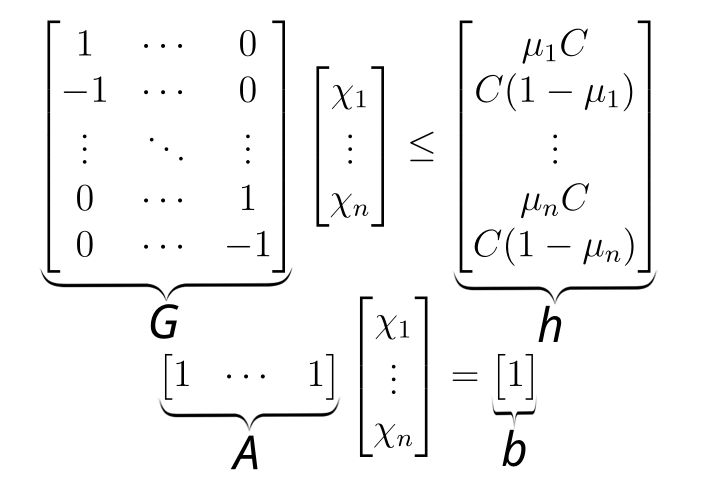
\includegraphics[width = 9 cm, height = 7 cm ]{images/Matrici_G_h_A_b.png}
    \centering
\end{figure}
% \begin{equation*}
%   \begin{bmatrix}
%       1 & \cdots & 0 \\
%       -1 & \cdots & 0 \\
%       \vdots & \ddots & \vdots \\
%       0 & \cdots & 1 \\
%       0 & \cdots & -1 \\
%   \end{bmatrix}
%   \begin{bmatrix}
%     \chi_1 \\ \vdots \\ \chi_n
%   \end{bmatrix}\leq
%   \begin{bmatrix}
%       \mu_1C \\
%       C(1-\mu_1)\\
%       \vdots\\
%       \mu_nC \\
%       C(1-\mu_n)\\
%   \end{bmatrix}
% \end{equation*}
% \begin{equation*}
%     \begin{bmatrix}
%         1 & \cdots & 1
%     \end{bmatrix}
%     \begin{bmatrix}
%         \chi_1 \\ \vdots \\ \chi_n
%     \end{bmatrix}=
%     \begin{bmatrix}
%         1
%     \end{bmatrix}
% \end{equation*}

\noindent \'E facile notare che il vettore delle variabili è definito da $\begin{bmatrix} \chi_1 \\ \vdots \\ \chi_n \end{bmatrix}$, e che i vincoli di diseguaglianza (\ref{eq:vincolo_1_forma_standard}) (\ref{eq:vincolo_2_forma_standard}) sono riportati in una singola matrice $G$ nella forma standard. Una volta ottenute queste matrici è facile trasporle in codice, utilizzando anche librerie come \textit{numpy}, così da permettere a CVXOPT di risolvere il problema.


\section{CVXPY}
L'ottimizzazione convessa ha molte applicazioni in diversi campi, tra cui anche il Machine Learning. Per utilizzare l'ottimizzazione convessa in un'applicazione spesso si ricorre a Solver che richiedono di porre il problema nella forma standard (come CVXOPT). Un alternativa è utilizzare un \textit{domain-specific language} (\textit{DSL}) per l'ottimizzazione convessa, che permette all'utente di specificare il problema in una maniera più naturale che rispecchia il linguaggio matematico, e successivamente questa specificazione viene convertita nella forma standard dal solver. CVX \cite{cvx} è un esempio tra i vari DSL esistenti.
CVXPY \cite{CVXPY_1} \cite{CVXPY_2} è un nuovo domain-specific language per i problemi di ottimizzazione convessa. Permette di esprimere il problema in un linguaggio naturale piuttosto che nella restrittiva forma standard richiesta da altri solver. \`E basato su CVX, ma introduce nuove funzionalità. CVXPY è semplicemente una libreria in Python che permette di combinare facilmente l'ottimizzazone convessa con le funzionalità ad alto livello di Python come ad esempio il parallelismo e la programmazione ad oggetti.

La sintassi di CVXPY è molto semplice, di seguito un'esemplificazione di come può essere costruito il nostro problema (\ref{eq:problema_finale_2}):
\begin{figure}[H]

    \begin{minted}{python}

        chis = Variable(n)
        objective = Minimize(quad_form(chis, P) - q.T @ chis)
        constraints = [G @ chis <= h, A @ chis == b]
        problem = Problem(objective, constraints)
        
        
        \end{minted}
\end{figure}

\noindent dove $q.T$ indica la trasposta della matrice $q$, e il simbolo $@$ è l'operatore di moltiplicazione tra matrici in Python. Come possiamo vedere, il problema diventa molto facilmente leggibile a livello utente, riuscendo ad individuare subito i protagonisti in gioco, quali le variabili, la funzione obiettivo, i vincoli e il problema finale. In realtà per quanto riguarda i vincoli, si possono riportare anche uno ad uno senza necessariamente ricorrere all'uso delle matrici.
Come impostazioni di default, CVXPY chiama il solver più appropriato per il problema. Nel caso della programmazione quadratica CVXPY utilizza OSQP \cite{osqp}, utilizzato principalmente anche negli esperimenti del Capitolo \ref{Captiolo 3}.






\section{Gurobi}
Gurobi \cite{gurobi} è un software commerciale, disponibile con licenza accademica, utilizzato per la risoluzione di problemi di ottimizzazione. Nato nel 2008, prende il nome dai suoi fondatori: Zonghao \textbf{Gu}, Edward \textbf{Ro}thberg and Robert \textbf{Bi}xby. Gurobi supporta una grande varietà di linguaggi di programmazione e modellazione, tra cui anche Python, al quale, grazie alle specifiche librerie, riesce a portare una nuova sintassi per creare modelli.
Infatti nel modulo \textit{optimization} di $\mu-learn$ \cite{mulearn_documentation} viene creato un ambiente che rappresenta perfettamente il problema matematico che vogliamo risolvere.
\begin{figure}[H]
    
\includegraphics[scale = 0.25]{images/gurobi.jpg}
    \centering
    \caption{Logo d Gurobi}
    \label{fig:gurobi_logo}
\end{figure}

\noindent A differenza dei solver gratuiti, Gurobi può essere più performante e veloce, sempre a seconda del contesto di ottimizzazione. Questo poiché spesso i solver gratuiti tendono a raggiungere i limiti di tempo previsti dal solver prima di aver effettivamente ottimizzato il problema, e quindi in alcuni casi dare risultati non propriamente corretti. Grazie all'affidabilità e la performance data da questo solver, viene utilizzato come metro di paragone per gli esperimenti del Capitolo \ref{Captiolo 3}.

\section{TensorFlow} %TensorFlow
TensorFlow \cite{tensorflow2015-whitepaper} è un software gratuito e open source utilizzato per machine learning e intelligenza artificiale. Inizialmente sviluppato dal team di Google Brain per un uso interno a Google, nel 2015 è stato rilasciato sotto una licenza Apache.
\begin{figure}[H]
    
\includegraphics[scale = 0.3]{images/TensorFlow_Logo.png}
    \centering
    \caption{Logo di TensorFlow}
    \label{fig:tensor_flow_logo}
\end{figure}

\noindent TensorFlow permette agli sviluppatori di creare dei \textit{grafi di dataflow}, ossia delle strutture che descrivono come i dati si muovono attraverso un grafo, o una serie di nodi. Ogni nodo nel grafo rappresenta un'operazione matematica, e ogni connessione tra i nodi è un array multidimensionale di dati, o meglio chiamati \textit{tensori}. TensorFlow fornisce tutto il necessario per la costruzione di questo grafo attraverso il linguaggio di programmazione Python. Nodi e tensori in TensorFlow sono oggetti in Python, e le applicazioni in TensorFlow sono applicazioni in Python.
Grazie a queste librerie è possibile costruire un modello per il nostro problema (\ref{eq:forma_standard}).

%\subsection{Rilassamento Lagrangiano}

%
%			CAPITOLO 3: esperimenti fatti

\chapter{Esperimenti}
\label{Captiolo 3}

Spiegare come sono stati costruiti ed eventuali esperimenti
Cercare un filo logico tra gli esperimenti, esperimenti miei e perché li ho fatti così.
\section{Esperimenti a confronto}
\subsection{CVXPY}
\subsection{CVXOPT}
\subsection{TensorFlow}
\subsubsection{Confronto con esperimenti precedenti}

\chapter{Conclusioni}
\label{Conclusioni}
Conclusioni e sviluppi futuri.

\chapter*{Ringraziamenti}
\label{Ringraziamenti}

%
%			BIBLIOGRAFIA
%

\bibliographystyle{IEEEtran}
\bibliography{biblio}
\addcontentsline{toc}{chapter}{Bibliografia}

\end{document}



